\section{Retrieve Process Design}
This section describes the design and behavior for restoring the archived project from the Synology back to the system
so that it can be used again using the MARS UI.   

\subsection{Decision of File Upload via File-svc}
\label{ssec:file}

\begin{figure}[H]
    \centering 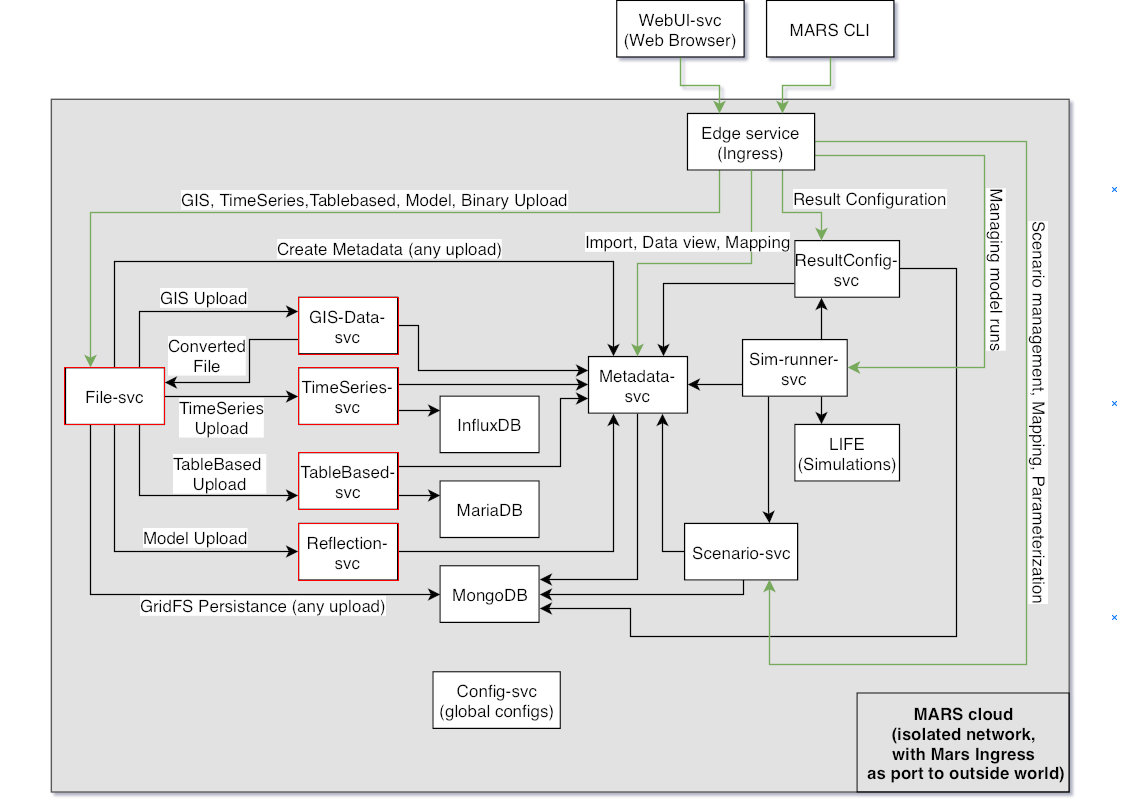
\includegraphics[scale=0.4]{grafiken/mars-cloud.png}
    \caption{File Upload in MARS Cloud \cite{MARSCLoud}}
    \label{fig:MARSCloud}
\end{figure}

Figure \ref{fig:MARSCloud} illustrates a file upload in the MARS cloud done at the time of writing this thesis. 
The MARS cloud consists of many 
microservices and databases at its disposal. It is a point of interest how the project is restored back as there are different possibilities for it. 
However, it is a requirement for the Archive service
to call the corresponding service to access, add, or modify the resources (Chapter \ref{chap:ReqAnalysis}). As mentioned in earlier chapters, the MARS system
has different types of files (e.g., models, timeseries, GIS) which are managed by their respective services. There are two different methods to upload a file 
and they are mentioned below :
\begin{enumerate}
 \item \textbf{Upload files via File-svc} The File-svc is a service which accepts all kind of inputs, i.e., GIS, models, timeseries. It communicates to the
 concerning service by checking the file type. This methodology is the only way possible through the UI for a file upload.   
 \item \textbf{Upload the respective file via its service} This method requires the Archive service to communicate with each service of the file type. 
The archive service can communicate to any service provided an endpoint (interface). Therefore, it is also possible to upload the different kinds of files using the
corresponding service instead of the File-svc. 
\end{enumerate} 

If a file type model is to be uploaded, an API call to the reflection service has to be made. Similarly, a GIS
file needs the GIS Data service.

The File-svc is an abstraction layer for uploading different types of files. This layer reduces the number of direct dependencies to the Archive
service because it does not call the other services directly. Choosing the File-svc also provides an additional advantage if a new file type is added in the future.
In this case, the archive service does not need to modify any code to upload the new file type. Given the reasons to have cohesion and easy maintenance, file uploads
via File-svc deemed to be a better choice. 

\subsection{Retrieve as an Atomic Action}
\begin{figure}[H]
    \centering 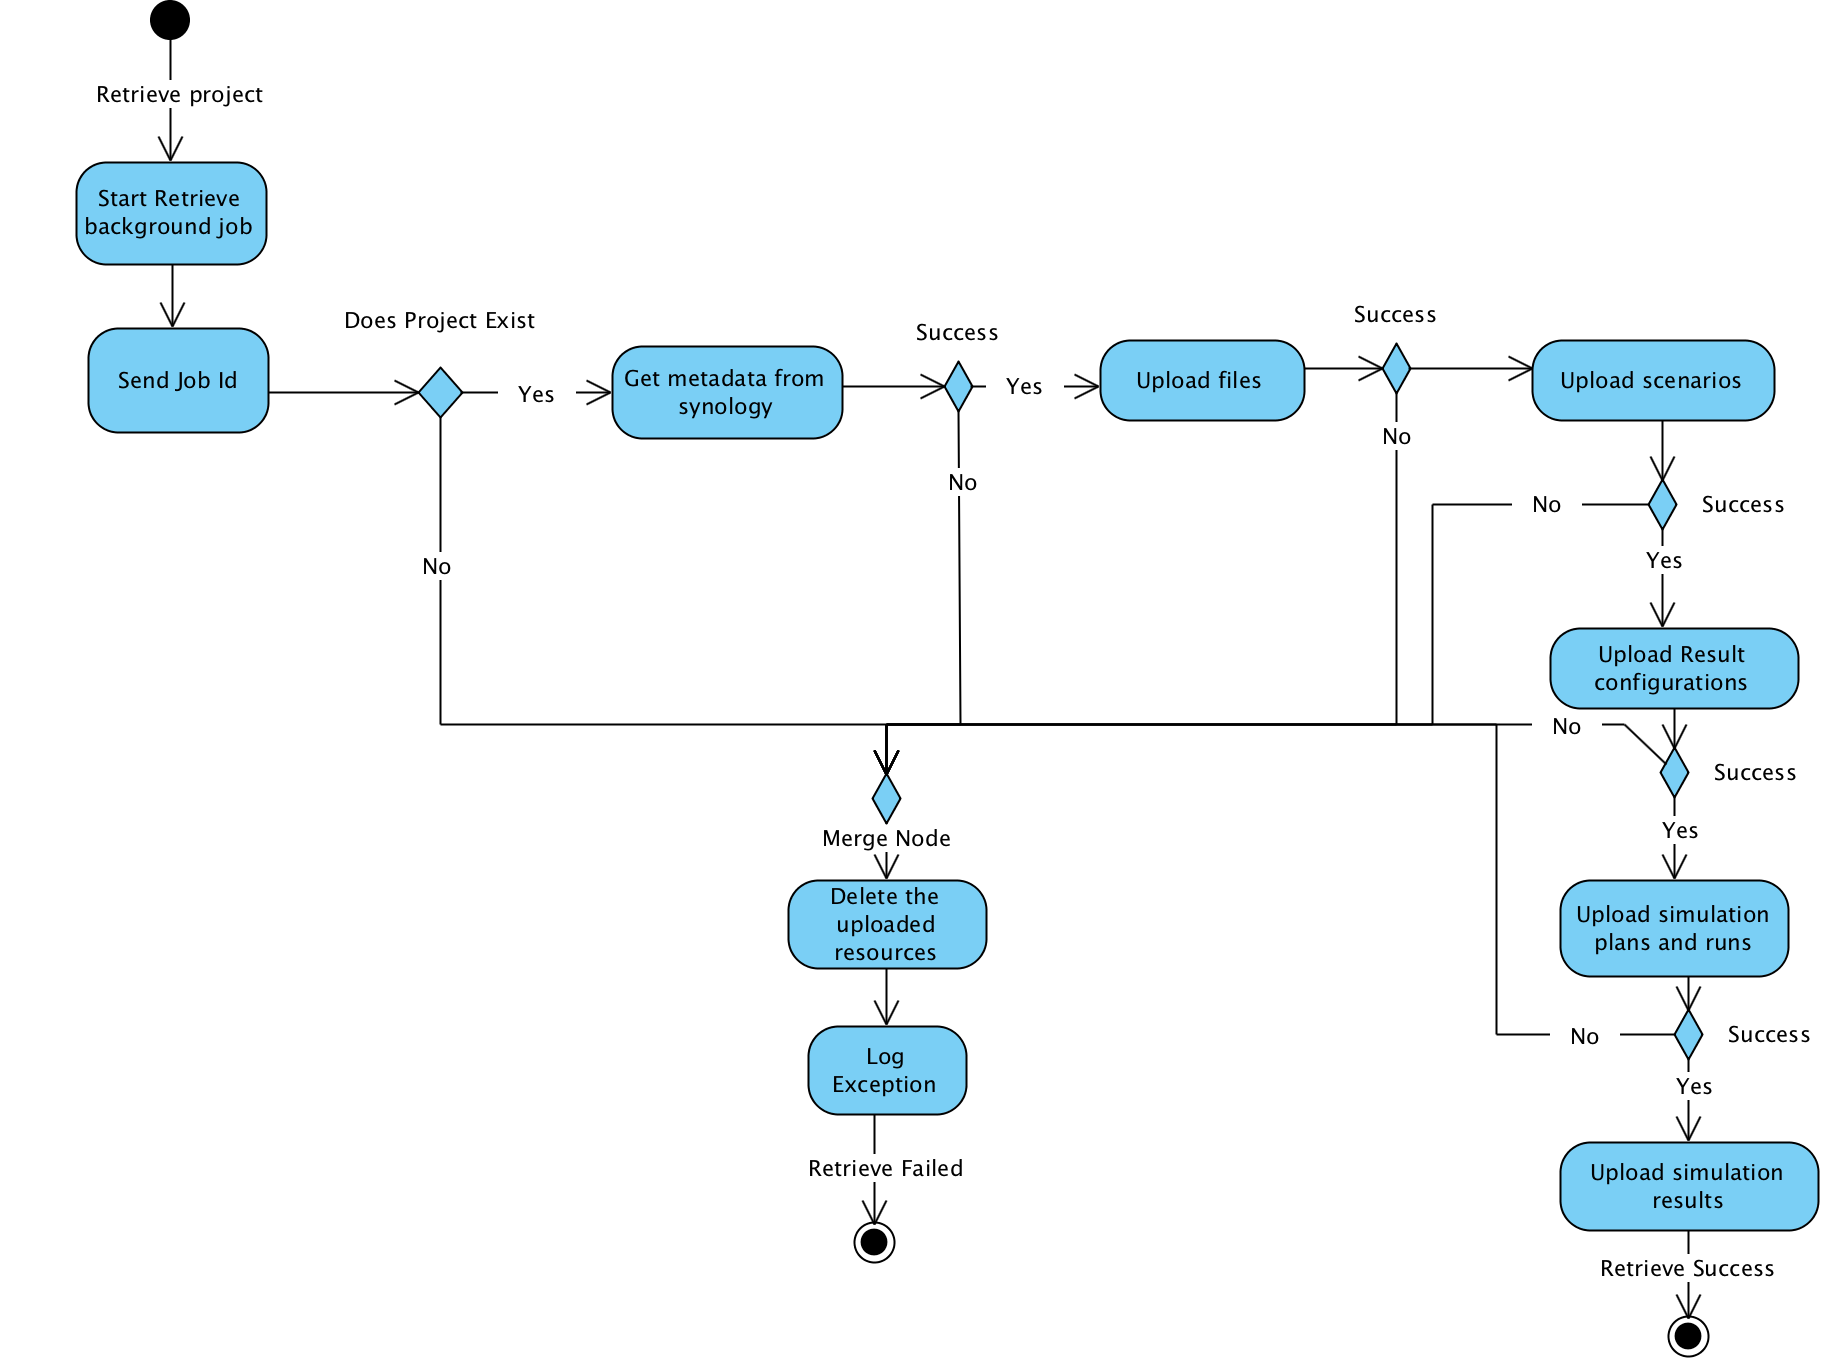
\includegraphics[scale=0.45]{grafiken/restoreActivity.png}
    \caption{Activity Diagram for retrieving a project}
    \label{fig:activityRestore}
\end{figure}

Figure \ref{fig:activityRestore} depicts the activity diagram for restoring a project. The retrieving process is also a background job due to the same reason
as for the archive, i.e., long running times. The first step after creating the retrieve job is to get the metadata from the Synology and then upload all the files.
All the files have to be finished uploading and processing; otherwise, the sequential steps would not have the references of the files. After all the uploads are complete,
the scenarios get the reference to the file id so that it could be uploaded. Following the scenarios, the result configurations are also uploaded for the corresponding models.
As the simulation plan is dependent on the scenario and the result configuration, this is the next resource which will be uploaded. Lastly, the simulation runs
and the simulation results are uploaded respectively. 

In case an error occurs, a Two-phase commit protocol \cite{atomic} is adopted. This strategy is taken into consideration to bring atomicity on decentralized data
as it tries to roll back if the distributed transaction fails.
Due to chances of failure, an incomplete data restore process could occur. In the MARS system, one cannot work with having
incomplete data since the resources are dependent upon each other. Having an atomic transaction for the retrieve process is a simple mechanism to overcome
this issue. In case of any failure during retrieval, the partially restored resources is deleted to make the retrieve process as an atomic action.

    \begin{figure}[H]
        \centering 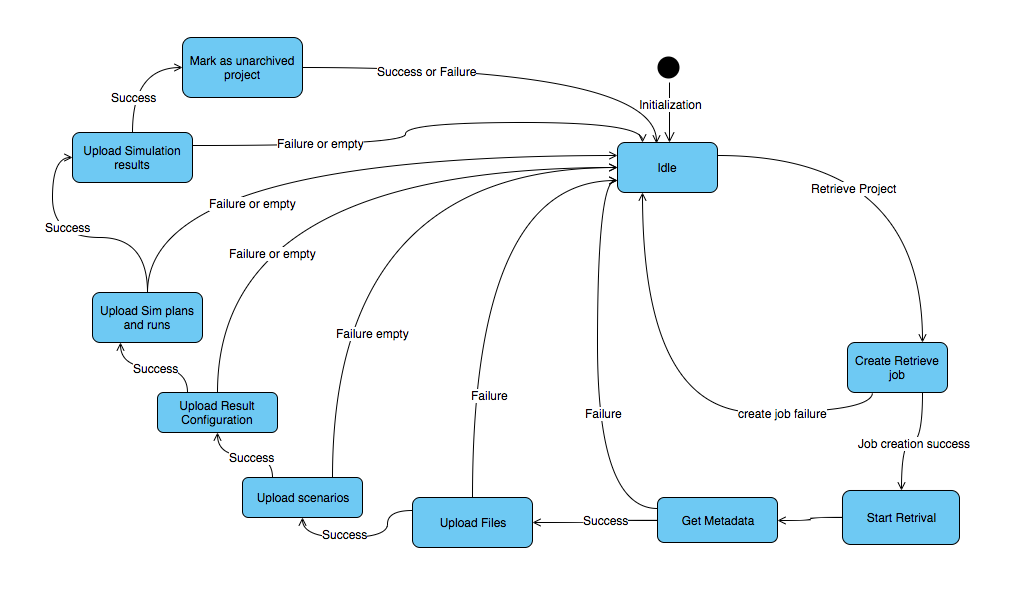
\includegraphics[scale=0.45]{grafiken/stateRestore.png}
        \caption{State Diagram of MARS project retrieval process considering empty states}
        \label{fig:stateRestore}
    \end{figure}

    Figure \ref{fig:stateRestore} illustrates the transitions that can occur in the retrieval process. The state diagram has a very similar procedure to the
    archive (Figure \ref{fig:stateArchive}), as both execute their actions in the same order. 
    Also, marking of the resources is not done before the start process in contrast to the archive, because data coherency issues are not present as the archived
    data is stored in a centralized storage, i.e., Synology which is accessed only by the Archive service.   

Figure \ref{fig:sequenceRestore} illustrates the sequence diagram for the retrieve process. The starting step is similar to the archive process 
as it makes a check if a process for the project is running or not. If a process is found running, then the restore process is denied. After a
successful job creation, the file metadata are fetched from the archives. Using them, the corresponding files are uploaded one after the other. 
In this process, different types of input files such as GIS, Timeseries, and models can be uploaded. Section \ref{ssec:file} mentions that the files are uploaded via
the File-svc (In the UI) which determines the input file type and forwards it for processing which requires additional time.
It is mandatory
that all the uploaded files have a "FINISHED" status which can be acknowledged by making another request using the data id received when uploading the file. 
Then, the restore file process waits until all the files have a "FINISHED" status. The request will be made in a designated time interval to avoid many
network calls. In the case of a status "FAILED," request timeouts, unknown status, and internal server error the whole restore process will halt. 
This step is necessary because the children resources cannot use the failed/incomplete files.

The next step is to get the scenario metadata. Restoring this data back to the system is not entirely straightforward because it needs some additional 
work to be done. 
The problem arises from the fact that the archived data have attributes like the resource id which changes as a new resource is uploaded. For more clarification, 
Listing \ref{lst:marsMetadata} presents an example of the archived metadata of a file. This resource is needed so that the restore process can determine the different 
attributes (e.g., title, project id) while uploading a new resource. During a new file upload 
its data id changes, as a new id is assigned by the File-svc (See Listing \ref{lst:marsNewMetadata}). 
This is a big problem because the other resources such as a scenario cannot be uploaded until it knows the new data id that was assigned to the model it 
depends on. Listing \ref{lst:marsScenario} shows the archived scenario which has a reference to the data id from the archived file metadata. 
This is only one example as many attributes must be considered. 

To solve this, a map using the old attribute as the key and the 
new id as the value is made (See Listing \ref{lst:marsMap}).
This way, while uploading, the scenario resource gets the new data id by searching the key, i.e., old id, from the map and replacing it during upload. 

Following a scenario upload, the other resources, i.e., result configuration, simulation plan, simulation run uses the same mapping strategy to replace 
the attributes required for restoring. 
Lastly, the simulation results will be restored from the archives. The restore process also waits until all the simulation runs are finished. Using a job id retrieved from the Database 
Utility service the status of the simulation restore can be known. Similar precaution for the file uploads are taken into consideration which prevents an infinite running
of this process.


\newpage
\begin{lstlisting}[caption={Snippet of archived MARS metadata resource}, language=json,firstnumber=1, captionpos=b, label={lst:marsMetadata}]
{
    "DataId":"7cae6055-d7fd-418e-9ba0-bdc2980ffb4c",
    "Title":"KNPGIS.zip",
    "Description":null,
    "ProjectId":"c5deed87-dd03-45c3-a0c4-fdf9f1a307a0",
    "UserId":"af7e045f-edf4-4df5-a9c8-6327186e6ddb",
    "Privacy":"PROJECT_PRIVATE",
    "State":"TO_BE_DELETED"
}
\end{lstlisting}

\begin{lstlisting}[caption={Snippet of the uploaded MARS metadata resource}, language=json,firstnumber=1, captionpos=b, label={lst:marsNewMetadata}]
{
    "DataId":"27765261-8a65-45ab-bdeb-db8b5b7f8f43",
    "Title":"KNPGIS.zip",
    "Description":null,
    "ProjectId":"c5deed87-dd03-45c3-a0c4-fdf9f1a307a0",
    "UserId":"af7e045f-edf4-4df5-a9c8-6327186e6ddb",
    "Privacy":"PROJECT_PRIVATE",
    "State":"TO_BE_DELETED"
}
\end{lstlisting}

\begin{lstlisting}[caption={Snippet of the archived MARS scenario resource}, language=json,firstnumber=1, captionpos=b, label={lst:marsScenario}]
{
    "MetaDataId":"7cae6055-d7fd-418e-9ba0-bdc2980ffb4c",
    "Description":"No description available.",
    "ClearName":"gis_vector_percipitation.zip",
    "AllowedTypes":["SHAPEFILE","GEOJSON"],
    "ParameterMapping":[]
}
\end{lstlisting}

\begin{lstlisting}[caption={The mapped key value attributes that the scenario metadata needs}, language=json,firstnumber=1, captionpos=b, label={lst:marsMap}]
{
    "7cae6055-d7fd-418e-9ba0-bdc2980ffb4c":"27765261-8a65-45ab-bdeb-db8b5b7f8f4"
}
    \end{lstlisting}

\begin{figure}[H]
    \centering 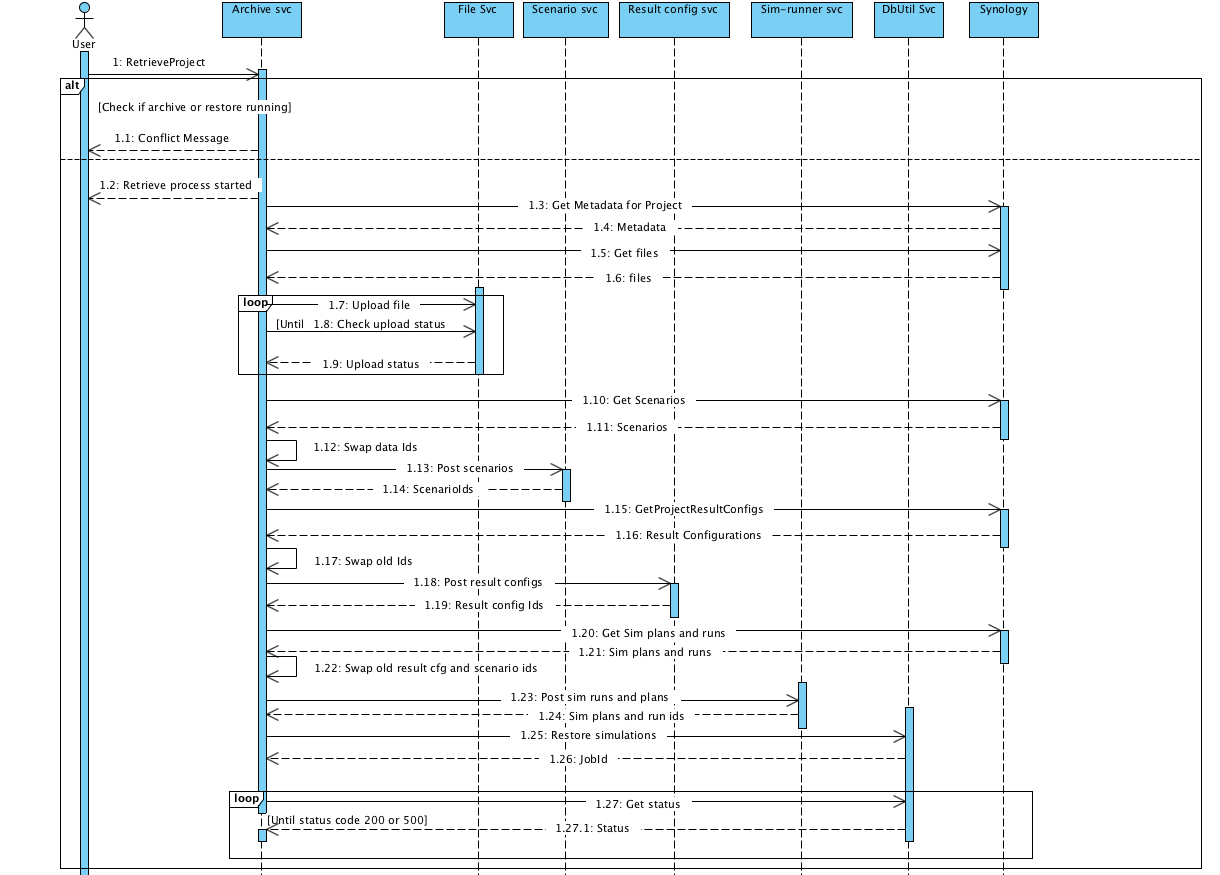
\includegraphics[scale=0.5, angle=90, origin=c]{grafiken/sequenceRestore.png}
    \caption{Sequence Diagram for the restore process}
    \label{fig:sequenceRestore}
\end{figure}
    
